%\section{Preprocessing}
The data we need to use is available from a database at the uva-bits website
\footnote{\url{https://public.flysafe.sara.nl/phppgadmin/} }. This database is often very slow 
and sometimes overloaded. This is why we downloaded all the data we required in one run. 
Before we can start in Matlab we preprocess this data to load only correct data in Matlab.

\subsection{Before Matlab}
\label{subsec:beforeMatlab}
Preprocessing of the data from a database dump is done in Java. Such data 
is checked for the following: 
\begin{enumerate}
    \item Is the data above the north sea? We are only interested in the birds behaviour 
    above the North Sea data from above the Wadden Sea or above Holland is removed.
    \item Is the data complete? If we require longitude and latitude every entry 
    without a value for these variables are excluded for the data for Matlab. 
    \item Is the data usable? Our method requires data to consist of long flights,
    not isolated data points. We call a sequence of useful data points a \textit{session}. 
    See subsection \ref{subsec:creatingSessions} for more details on sessions and how
    they are created.
\end{enumerate}

Furthermore the date time was rewritten to a time stamp. We wanted to time stamps to be 
as small as possible so instead of using standard Unix time we use \textit{seconds passed
since 
January 1 2008}. This could be done because the earliest data in the database was from after
this date. 

\subsection{Creating Sessions}
\label{subsec:creatingSessions}
As discussed in subsection \ref{subsec:beforeMatlab} a part of the script involves 
dividing the data points up in to sessions. Isolated data points should be excluded. 
When there is a too big of a time span between two data points, a new sessions should be 
created. Furthermore a session should not be too short and it should not contain too few
data points (the resolution of data points per minutes should be within a range of 
acceptable values). 

This has to be done because our method involves the detection of clusters and this
can only be done with an actual flight of the bird. 

We use the following parameters to define which sequences of data points can be called sessions: 
\begin{itemize}
    \item Total minutes described. This is currently set to \minimumSessionLengthMinutes minutes. Less than \minimumSessionLengthMinutes minutes of flight is not interesting.
    \item Range of resolution. We can filter for a range of data points per minutes. There is
no way to extract the same amount of information from low resolution data as from high 
resolution data. This is why we filter out the low resolution data. The resolution 
we now use is \resolutionRange data points per minute.
    \item The maximum amount of minutes between two data points. Sometimes the device
can't update at the preferred moments. We end a session at such a point because we need
the information of what the bird is doing \emph{all the time} to be able to cluster 
acceptably. 
\end{itemize}

A lot of data is thrown away because of these filters. About \textbf{90\%} of the data 
from the database is data we can not use because it is not above the North Sea, incomplete
or not in context with other data points (can't be put in a session). The parameters are  
responsible for 
some of these percentages. We chose these parameters because our client told us it is better
to use less data which we know is good than use more data which can be questionable. In 
other words, it does not matter that much that we end up with less data to learn from and
to classify. 

\subsection{GPS and accelerometer data}
\label{subsec:gpsAndAccelerometerData}
There is also a difference between GPS data and accelerometer data, namely: there are a lot
more GPS data points then there are accelerometer data points
(It seems that \textbf{25\%} of the GPS data also has accelerometer data).
This is why we create 
sessions using only
the GPS data. We later match the accelerometer data to GPS sessions. 

The output of this
script is $N$ comma separated GPS session files (containing GPS data that together makes
a session) and $M$ (with $0 <= M <= N$) comma separated accelerometer data files. Matlab
can easily match GPS data with accelerometer data using these files. 

 \subsection{Normalizing Height}
 The best way to distinguish flying from floating is, of course, by the height of the bird. Unfortunately the height calculated by the GPS is very unreliable\footnote{this has to do with triangularisation and switching of satellites}. The absolute value of the height is unusable (often the bird is flying 100 meters below the surface), but changes in height can be used on short intervals. In the preprocessing we will remove outliers from this data (large shifts in height, often because of a satellite switch) so we can later try to create features from it.

\begin{figure}[htb!]
 \begin{center}
 \subfig {
  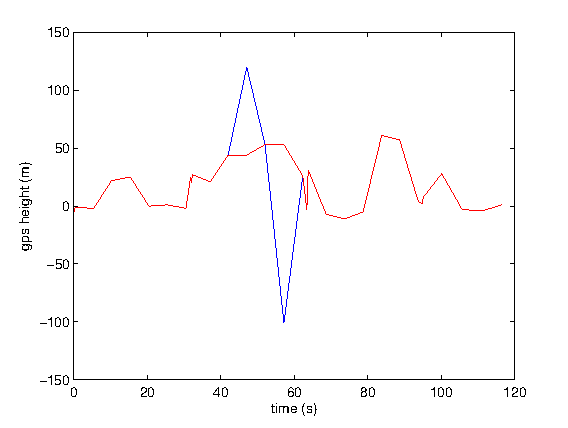
\includegraphics[scale=0.5]{heightnorm9}
 }
 \subfig {
  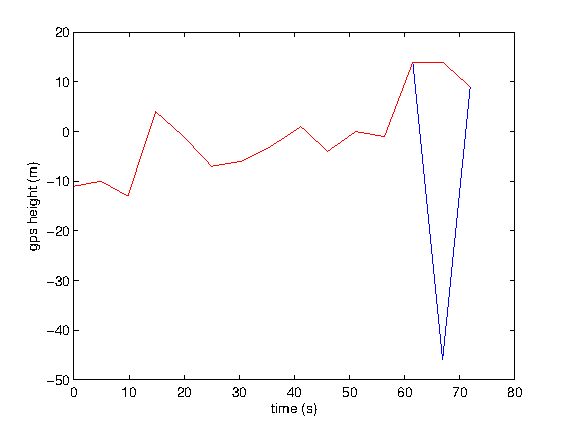
\includegraphics[scale=0.5]{heightnorm10}
 }
 \end{center}
 \caption{The blue line is the height from raw gps data, the red line is the normalized height.}
 \label{fig:heightnorm}
\end{figure}

We currently flatten height points in a cluster that are more than $3$ times the standard deviation away from the mean, which is a commonly used method\footnote{Sources:\\ http://en.wikipedia.org/wiki/Outlier\\ http://www.mathworks.nl/help/techdoc/data\_analysis/f0-7275.html} . Figure \ref{fig:heightnorm} shows some results. There is still a lot of noise left in the data, more experimenting will be needed to find a solution for this.




